% $Id: ESMF_archdoc.tex,v 1.3 2002/08/08 17:47:28 cdeluca Exp $

%
\documentclass[]{article}

\usepackage[dvips]{graphics,color}
\usepackage{epsf}
\usepackage{html}
\usepackage[T1]{fontenc}

\textwidth 6.5in
\textheight 8.5in
\addtolength{\oddsidemargin}{-.75in}

\begin{document}

\bodytext{BGCOLOR=white LINK=#083194 VLINK=#21004A}

\begin{titlepage}

\begin{center}
{\Large Earth System Modeling Framework } \\
\vspace{.25in}
{\Large {\bf ESMF Architecture}} \\
\vspace{.25in}
{\large {\it DRAFT}}
\vspace{.5in}
\end{center}

\begin{latexonly}
\vspace{5.5in}
\begin{tabular}{p{5in}p{.9in}}
\hrulefill \\
\noindent {\bf NASA High Performance Computing and Communications Program} \\
\noindent Earth and Space Sciences Project \\
\noindent CAN 00-OES-01 \\
\noindent http://www.esmf.ucar.edu \\
\end{tabular}
\end{latexonly}

\end{titlepage}

\tableofcontents

\newpage

%\section{Overview}

{\it 
In this section, we describe: 
\begin{itemize}
\item the goals and unique role of ESMF in Earth science;
\item the relevant features of the problem domain that ESMF encompasses; and
\item the key design features that are derived from the requirements of the ESMF domain and 
enable the ESMF to satisfy its goals. 
\end{itemize}
}

The {\bf Earth System Modeling Framework (ESMF)} is a software toolkit that increases 
software reuse, component interoperability, performance portability, and ease of use in 
Earth science applications.  The focus on Earth systems - a diverse but bounded domain - is 
critical to the ability of the ESMF to achieve its goals.  This is where the ESMF's value and 
capability come from - enabling interoperability but able to retain some efficiency and structure 
because the domain is bounded.  The scope is also unique - there are larger projects and smaller 
projects, but only ESMF spans institutions that are all interested in collaboration. The fifteen 
initial testbeds for the ESMF represent a wide range of research and operational applications in 
climate, weather, and data assimilation \cite{ref:models}.  Thus the ESMF must efficiently 
support a variety of grids, programming paradigms, and computing platforms.  However, the ESMF 
domain is restricted enough to allow the creation of specific data and control constructs.  A 
challenge of the project is to support high-performance operations in the face of the generality 
that's required.  Commonality in applications can be found at both the {\bf infrastructure} 
level, in model development tools for communication, I/O, time management, and other basic 
functions; and at the {\b superstructure} level, in an architecture and standards for 
combining geophysical components into applications.

The ESMF design is rooted in the requirements and characteristics of the applications that 
the framework must support.  In the sections below, these characteristics are described.  
Then we describe the major architectural implications that spring from the nature of the 
domain.

The key characteristics of the Earth science code that the ESMF must address are as follows.
\begin{enumerate}

\item Applications contain sets of complex software components that represent different 
physical domains, such as land, ocean, atmosphere and sea ice.  Other components may perform 
data assimilation or analysis.  These components are "coupled" so that the output fields of 
some of the components are used 
as the input fields for other components.  Coupling may include data transfers, unit 
conversions, flux 
calculations, regridding, data transfers, and other transformations.  The software that 
couples components is often viewed as a component itself.  

\item The same models or components may be run in a variety of configurations.  Scientists 
may swap in
alternative implementations of a domain or function in order to create new applications 
(e.g., different 
ocean models, different dynamical cores); may use different subsets and combinations 
of a particular set of 
components (e.g., an atmospheric model may be run with an ocean model for a 
hurricane application, and 
with a full complement of land, ocean, and sea ice models for a climate simulation); may 
run ensembles of the same component; and as a matter of course attempt endless variations 
and combinations of these research strategies.

\item Applications run on a variety of parallel computing systems and require high performances. 

\item Applications have many diverse users, from graduate students to software engineers 
to .  Applications are under continuous scientific development, and scientists and developers 
frequently wish to modify and update the code.

\end{enumerate}

The characteristics above inform a software architecture.  The key architectural features 
of ESMF are described below.

\begin{description}
\item[Component-based architecture]  Applications running under ESMF are organized as sets of 
interacting {\bf Components}.  A Component is
a software representation of some domain or function; for example, a land model or data 
assimilation 
system.  All Components share common behavior in ESMF.  This architectural model lends itself 
naturally to systems whose functionality is segregable.

\item[Types of Components]  ESMF Components fall into a number of categories.  The two primary 
types are Gridded 
Components ({\tt ESMF\_GridComp}) and ESMF Coupler Components ({\tt ESMF\_CplComp}).  A 
Gridded Component represents 
a physical domain that contains fields discretized on a grid.  A Coupler Component performs the operations required for two or more components to interact with each other.

\item[Local communication]

One of the important features of the ESMF architecture is that all communication between 
Gridded Components is 
local.  Another way of stating this is that all inter-component communication is mediated 
by a Coupler Component.    
\end{description}























%\section{Requirements}
%% $ Id: $

Here we describe the requirements that apply to the whole body of 
ESMF software.  We adopt the standard requirements format described in 
the \htmladdnormallink{ESMF Software Developer's Guide}{http://www.esmf.ucar.edu/esmf\_docs/dev\_guide}.  The abbreviation used to identify
these General Requirements is {\bf GR}. The requirements
are drawn from the applications and user needs from ESMF project 
participants \cite{ESMFWEBSITE}, from community feedback and from background analysis carried out by the NASA
computational technologies group \cite{WOM2002}.

\req{Computational requirements}

\sreq{Language bindings}
ESMF software shall support the following language bindings:

\ssreq{Fortran 90 interface}
\begin{reqlist}
{\bf Priority:} 1. \\
{\bf Source:} All codes except GFDL-HIM require F90 interfaces. \\
{\bf Status:} Approved-1. \\
{\bf Verification:} Interface inspection (verification
  checklist will include array dimension information and 
  optional argument handling).
\end{reqlist}

\ssreq{C++ interface}
\begin{reqlist}
{\bf Priority:} 1. \\
{\bf Source:} GFDL-HIM. \\
{\bf Status:} Approved-1. \\
{\bf Verification:} Interface inspection (verification
  checklist will include array dimension information and 
  optional argument handling).\\
{\bf Notes:} Handling of Try/Catch exception handling and 
error signal propogation over the C/C++ Fortran boundary 
will need to be addressed in the preliminary design and
implementation prototyping.
\end{reqlist}

\ssreq{C interface}
\begin{reqlist}
  {\bf Priority:} none \\
  {\bf Source:} GFDL-HIM. \\
  {\bf Status:} Rejected. \\
  {\bf Notes:} There will be a single interface serving C and C++
  applications. This C/C++ interface will be sufficient so the C only
  interface has been rejected.
\end{reqlist}

\sreq{Platforms}
The ESMF shall operate on the following platforms:

\ssreq{IBM SP}
\begin{reqlist}
{\bf Priority:} 1-approved. \\
{\bf Source:} NCAR, NCEP. \\
{\bf Status:} Approved-1. \\
{\bf Verification:} Unit test and system test.
\end{reqlist}

\ssreq{SGI Origin}
\begin{reqlist}
{\bf Priority:} 1-approved. \\
{\bf Source:} GFDL, LANL, NCAR, DAO.  May be part of ESMF testbed system. \\
{\bf Status:} Approved-1. \\
{\bf Verification:} Unit test and system test.
\end{reqlist}

\ssreq{Compaq ES}
\begin{reqlist}
{\bf Priority:} 1. \\
{\bf Source:} NSIPP, DAO.  May be part of ESMF testbed system. \\
{\bf Status:} Approved-1. \\
{\bf Verification:} Unit test and system test.
\end{reqlist}

\ssreq{PC Linux platforms (including cluster)}
\begin{reqlist}
{\bf Priority:} 1. \\
{\bf Source:} MIT.  Required for optional cluster milestones. \\
{\bf Status:} Approved-1. \\
{\bf Verification:} Unit test and system test.
\end{reqlist}

\ssreq{Sun-Solaris}
\begin{reqlist}
{\bf Priority:} 1. \\
{\bf Source:} NCAR. \\
{\bf Status:} Approved-1. \\
{\bf Verification:} Unit test and system test.
\end{reqlist}

\ssreq{Vector machines running Unix}
\begin{reqlist}
{\bf Priority:} 2. \\
{\bf Source:} NCAR. \\
{\bf Status:} Approved-2. \\
{\bf Verification:} Unit test and system test.
\end{reqlist}

% $Id: ESMF_buildreq.tex,v 1.1 2003/01/27 20:30:14 flanigan Exp $

\sreq{Build}

\ssreq{Build system will use GNU Make}
The build system will utilize the Build program Make from
GNU.  Other vendors' make programs will not be supported.
\begin{reqlist}
{\bf Priority:} 1. \\
{\bf Source:} ESMF/CSS. \\
{\bf Status:} DRAFT. \\
{\bf Verification:} Makefiles will test make being used and generate
warning if GNU make not being used.
\end{reqlist}

\ssreq{Library Archive Files}
Both .a and .so archive files will be created by the 
build system.
\begin{reqlist}
{\bf Priority:} 1. \\
{\bf Source:} ESMF/CSS. \\
{\bf Status:} DRAFT. \\
{\bf Verification:} After build linkable .a and .so files will exist.
\end{reqlist}

\ssreq{Targets}
The build system tasks will be controlled with a series of
makefile targets.  These targets will only be available 
in the makefile located in \$ESMF\_DIR.  These targets will be:
\begin{description}
\item[all] Builds all libraries, test programs and documentation.
\item[install] Installs ESMF products.
\item[build\_libs] Builds .a and .so archive files.
\item[build\_c] Compiles all c and c++ source code.  (Create libs ?)
\item[build\_fortran] Compiles all FORTRAN source code (Create libs ?)
\item[build\_test] Compiles and links the test program source code.
\item[docs] Builds all formats of the documentation.
\item[dvi] Builds dvi documentation files.
\item[pdf] Builds pdf documentation files.
\item[html] Builds html documentation files.
\item[clean] Removes all products for current architecture.
\item[clobber] Removes all products for all architectures.
\end{description}

\begin{reqlist}
{\bf Priority:} 1. \\
{\bf Source:} ESMF/CSS. \\
{\bf Status:} DRAFT. \\
{\bf Verification:} Review
\end{reqlist}

\ssreq{Local Builds}
Builds within the current working directory will be
accomplished with a build to the target ``local''.
Only build tasks within and below the CWD will be
processed.  
\begin{reqlist}
{\bf Priority:} 1. \\
{\bf Source:} ESMF/CSS. \\
{\bf Status:} DRAFT. \\
{\bf Verification:} Review
\end{reqlist}


\ssreq{Internal Documentation}
Documentation will exist to explain the structure and 
internal workings of the Build System.
\begin{reqlist}
{\bf Priority:} 1. \\
{\bf Source:} ESMF/CSS. \\
{\bf Status:} DRAFT. \\
{\bf Verification:} Less Confusion.
\end{reqlist}

\ssreq{User Documentation}
Documentation will exist to cover steps needed to build ESMF
and EVA source trees.  This will include procedures for 
changing the compile and link options.
\begin{reqlist}
{\bf Priority:} 1. \\
{\bf Source:} ESMF/CSS. \\
{\bf Status:} DRAFT. \\
{\bf Verification:} ESMF Group Review
\end{reqlist}

\ssreq{Developer Documentation}
Documentation will exist to cover steps needed to add source
code to the ESMF and EVA source trees.
\begin{reqlist}
{\bf Priority:} 1. \\
{\bf Source:} ESMF/CSS. \\
{\bf Status:} DRAFT. \\
{\bf Verification:} ESMF Group Review
\end{reqlist}

\ssreq{EVA Builds}
The same makefile targets, variables and rules
will be used by the EVA build system.
\begin{reqlist}
{\bf Priority:} 1. \\
{\bf Source:} ESMF/CSS. \\
{\bf Status:} DRAFT. \\
{\bf Verification:} EVA test programs.
\end{reqlist}


\ssreq{Concurrent Builds}
The same set of files can be used for builds on separate 
system architectures concurrently.
\begin{reqlist}
{\bf Priority:} 2. \\
{\bf Source:} ESMF/CSS. \\
{\bf Status:} DRAFT. \\
{\bf Verification:} Test.
\end{reqlist}

\ssreq{Dependency Checking}
The build system will take into account the dependencies 
between source code files and build products.  
\begin{reqlist}
{\bf Priority:} 2. \\
{\bf Source:} ESMF/CSS. \\
{\bf Status:} DRAFT. \\
{\bf Verification:} Script
\end{reqlist}

\ssreq{Automatic Dependency Generation}
The build system will scan source code files to 
generate dependency lists.
\begin{reqlist}
{\bf Priority:} 3. \\
{\bf Source:} ESMF/CSS. \\
{\bf Status:} DRAFT. \\
{\bf Verification:} Script
\end{reqlist}

\ssreq{Log Files}
Status and error log files will be generated by 
the build system.
\begin{reqlist}
{\bf Priority:} 3. \\
{\bf Source:} ESMF/CSS. \\
{\bf Status:} DRAFT. \\
{\bf Verification:} Visual Check
\end{reqlist}

\ssreq{Configuration Checking}
The build system will check for the required system 
libraries and utilities.
\begin{reqlist}
{\bf Priority:} 3. \\
{\bf Source:} ESMF/CSS. \\
{\bf Status:} DRAFT. \\
{\bf Verification:} Script
\end{reqlist}

\ssreq{Easily customize build for local machine}
The ESMF shall have the ability to easily customize the build environment. 
System libraries that are required can be set easily, without modifying 
the build files directly. If the paths to required system libraries 
are not provided or incorrect the build system will let the user know 
how to set them and die gracefully.
\begin{reqlist}
{\bf Priority:} 2. \\
{\bf Source:} CCSM-CPL. \\
{\bf Status:} Approved-2. \\
{\bf Verification:} Set library paths correctly and incorrectly and test that 
the build acts appropriately.
\end{reqlist}


\sreq{Performance} \label{perf}
Fully compliant adoption of the framework shall not increase the execution time 
of the milestone G codes, which are maintained and developed outside the 
framework throughout the project, by more than 10\% on scalar 
architectures within their scalable range.
\begin{reqlist}
{\bf Priority:} 1. \\
{\bf Source:} Required for Milestone G. \\
{\bf Status:} Approved-2. \\
{\bf Verification:} Demonstrate with NCEP analysis and MITgcm ocean.
\end{reqlist}

\sreq{Precision} ESMF will provide methods for applications using
default integers and floating-point numbers at either 32-bit or 64-bit
precision.

\begin{reqlist}
  {\bf Priority:} 1. \\
  {\bf Source:} DAO, NCEP. \\
  {\bf Status:} Approved-1. \\
  {\bf Verification:} Interface inspection (verification 
  checklist will include array dimension information and
  optional argument handling) , code inspection, unit
  test, system test. \\
  {\bf Notes:}
  \begin{enumerate}
  \item While it is technically possible through overloading to allow
    argument lists to contain arbitrary combinations of 32-bit and
    64-bit quantities, this Requirement only calls for a uniform
    application-wide word length for integers and FP numbers to be
    supported.
  \item There may be individual operations within ESMF that explicitly
    call for transformations between 64-bit and 32-bit quantities.
    Those will appear as individual requirements.
  \end{enumerate}
\end{reqlist}

\sreq{Runtime configurability} The ESMF shall allow the user to set
certain application parameters at runtime.
\begin{reqlist}
{\bf Notes:} There are many runtime configurable parameters that 
need to be set for codes operating as framework components.
The sub-requiremente listed here \ref{req:gr:Configurable_decomposition} - 
\ref{req:gr:Configurable_paths_and_directories} are some, but not all of these.
\end{reqlist}

\ssreq{Configurable decomposition} ESMF shall allow domain
decomposition and assignment of domains to processors, nodes, and/or
threads to be configurable at runtime.  The choice of parallelization
mechanism (message passing/multithreading/combination) must be
configurable at runtime.
\label{req:gr:Configurable_decomposition}
\begin{reqlist}
{\bf Priority:} 1. \\
{\bf Source:} CAM-EUL. \\
{\bf Status:} Approved-1. \\
{\bf Verification:} System test.
\end{reqlist}

\ssreq{Configurable resolution}
ESMF shall allow model resolution to be configurable at runtime.
\begin{reqlist}
{\bf Priority:} 1. \\
{\bf Source:} all codes. \\
{\bf Status:} Approved-1. \\
{\bf Verification:} System test.
\end{reqlist}

\ssreq{Configurable paths and directories}
ESMF shall allow input and output paths and directories to be specified
at runtime.
\label{req:gr:Configurable_paths_and_directories}
\begin{reqlist}
{\bf Priority:} 1. \\
{\bf Source:} all codes. \\
{\bf Status:} Approved-1. \\
{\bf Verification:} System test.
\end{reqlist}

\sreq{Bit-reproducibility}

Bitwise identical results between two runs is an important feature for
deterministic execution, as well as for debugging and maintenance.
This is not possible to enforce across platforms, at different levels
of compiler optimization, or even different versions of the same
compiler. Within these constraints, ESMF shall provide varied levels
of bit-reproducibility:

\ssreq{Parallel bit-reproducibility}

An execution mode will be provided which allows an ESMF-based model to
return bitwise identical results from the same executable at different
processor counts, or different parallelism options. This execution
mode is not subject to the performance requirement of Section~\ref{perf}.

\begin{reqlist}
{\bf Priority:} 1. \\
{\bf Source:} all JMC codes. \\
{\bf Status:} Approved-1. \\
{\bf Verification:} System test.
\end{reqlist}

\ssreq{Bit-reproducibility on identical configurations}

The \emph{default} execution mode will allow an ESMF-based model to
return bitwise identical results from the same executable at the same
processor count, with the same parallelism options. This mode
\emph{is} subject to the performance requirement of
Section~\ref{perf}.

\begin{reqlist}
{\bf Priority:} 1. \\
{\bf Source:} all codes. \\
{\bf Status:} Approved-1. \\
{\bf Verification:} System test.
\end{reqlist}

\ssreq{Non bit-reproducing fast option}

If a performance enhancement may be had by waiving the default
requirement above, this will be made available in a special execution
mode. In this mode, even two runs at the same processor count, with
the same parallelism options, may not return bitwise identical
results.

\begin{reqlist}
{\bf Priority:} 2. \\
{\bf Source:} NCEP, HIM. \\
{\bf Status:} Approved-2. \\
{\bf Verification:} System test.
\end{reqlist}

\sreq{Error handling}
The ESMF shall be instrumented for error handling consistly across the
framework.  The user shall receive ample information on errors including
comprehensive error logging.
\label{req:gr:error_handling}
\begin{reqlist}
  {\bf Priority:} 1. \\
  {\bf Source:} Required by all codes. \\
  {\bf Status:} Approved-1. \\
  {\bf Verification:} Interface inspection (verification
  checklist will include array dimension information and 
  optional argument handling), code inspection, unit
  test, system test.
  {\bf Notes} Components will be required to use ESMF error
handling utilities for fatal erros to be classified as 
{\it well-behaved} ESMF components.
\end{reqlist}

\ssreq{Parallel race-condition error handling}
Error handling code to detect race-conditions and other problems associated 
with parallelism shall be included.
\label{req:gr:error_handling}
\begin{reqlist}
  {\bf Priority:} 1. \\
  {\bf Source:} Required by all codes. \\
  {\bf Status:} Approved-1. \\
  {\bf Verification:} System test.
  {\bf Notes} This could be achieved through assertions and ordering/bookeeping
counters on messaging on communication operations.
\end{reqlist}

\ssreq{Debug mode for component comparison}
It shall be possible to run two instances of a component instrumented 
with debug directives and compare results on the fly.  When 
the results are the same no messages are produced; when they differ
informative messages are generated.
\begin{reqlist}
  {\bf Priority:} 2. \\
  {\bf Source:} Generated by NOAA FSL, desired by GFDL. \\
  {\bf Status:} Approved-2. \\
  {\bf Verification:} System test.
  {\bf Notes} See community requirements number 1003.
\end{reqlist}

\sreq{Modularity}
Layers of the framework will be designed to adapt to restructuring of
other parts of the framework and user-supplied components.  For
example, the coupling layers should be able to adapt to different
implementations and data structures of component models.
A modular design and implementation approach must be used that ensures
parts of the framework are independent of one another and can be 
developed concurrently.
\begin{reqlist}
{\bf Priority:} 1. \\
{\bf Source:} Required for interoperability Milestones I and J. \\
{\bf Status:} Approved-1. \\
{\bf Verification:} Interoperability experiments and incremental
adoption demonstrations by deployment teams.\\
{\bf Notes:} Good encapsulation, modular design and clean interfaces are critical to the
maintenance of models built with the framework. Framework classes, modules and algorithms must be
easy to adapt to take advantage of new techniques that are developed
by the Earth science community and added to the framework.
\end{reqlist}

\sreq{Extensibility} The ESMF framework must allow extensions both
for core suppport capabilities and through plug-in components.
Framework classes, modules and algorithms must be easily extensible
to allow additional functionality to be added for supporting new components
like atmospheric chemistry, carbon cycle, etc...
\begin{reqlist}
{\bf Priority:} 1. \\
{\bf Source:} All codes\\
{\bf Status:} Approved-2. \\
{\bf Verification:} Milestone demonstrations of migration
of more than twelve major applications and six styles of gridding.\\
{\bf Notes:} It is important that appropriate abstract interfaces and polymorphic 
methods are used to ensure adding new methods, grids, algorithms and data structures
can be easily done. This will facilitate building new types of models that are not
currently available.
\end{reqlist}

\sreq{Flexibility} The ESMF framework will be flexible and will
be suited to a wide range of Earth science applications and a broad span
of target hardware. Framework classes, modules and algorithms must be flexible and
provide options to support both efficiency and accuracy.
\begin{reqlist}
{\bf Priority:} 1. \\
{\bf Source:} All codes\\
{\bf Status:} Approved-1. \\
{\bf Verification:} Milestone demonstrations of migration
of more than twelve major applications on several different
platforms covering a wide variety of science scenarios
that span research to operational forecasting.
\end{reqlist}

\sreq{Documentation} An exhaustive collection of documentation
to support ongoing evolution of ESMF is required. The framework must be 
fully documented, easily understandable and well supported.
\begin{reqlist}
{\bf Priority:} 1. \\
{\bf Source:} All codes\\
{\bf Status:} Approved-1. \\
{\bf Verification:} Compliance with software developers guide.
{\bf Notes:} The Software Developers Guide specifies a suite of documents 
that will be produced.
\end{reqlist}

\sreq{Systematic build, test, packaging} A systematic scheme for disseminating
stable, versioned software and for gathering and tracking defects is required.
The framework should be delivered to developers using the standard packaging
utility for the supported platforms.
\begin{reqlist}
{\bf Priority:} 1. \\
{\bf Source:} All codes\\
{\bf Status:} Approved-1. \\
{\bf Verification:} Compliance with software developers guide.
{\bf Notes:} The Software Developers Guide specifies a versioning
schemes that will be used, release schedules and mechanisms for monitoring
and managing product quality.
\end{reqlist}

\sreq{Compatability with batch execution}
\begin{reqlist}
{\bf Priority:} 1. \\
{\bf Source:} All codes\\
{\bf Status:} Approved-1. \\
{\bf Verification:} Milestone demonstrations.\\
{\bf Notes:} In this mode, all input and output data are read and stored
directly from file. This will be the standard mode of operations used by
many ESMF applications.
\end{reqlist}

\sreq{Compatability with interactive execution}
\begin{reqlist}
{\bf Priority:} 1. \\
{\bf Source:} All codes\\
{\bf Status:} Approved-1. \\
{\bf Verification:} Milestone demonstrations.\\
{\bf Notes} This mode allows rapid testing of new features and debugging.
A trace mode which allows program excution to be logges in detail,
but at the expense of reduved performance, is useful in this mode.
Future extensions could include elements of computatinal steering
in which program progress can be monitored and directed
interactively.
\end{reqlist}

\sreq{Compatability with ensemble methods}
\begin{reqlist}
{\bf Priority:} 1. \\
{\bf Source:} All codes\\
{\bf Status:} Approved-1. \\
{\bf Verification:} Milestone demonstrations.\\
{\bf Notes:} Ensemble methods require multiple instances of
the same base component, generally with slight parametric variations.
The ability to spawn numerous ensembles and then collect together
results for automated processing, such as covariance calculation, 
is a basic requirement. A general mix of concurrent and sequential ensemble 
member execution must be supported.
\end{reqlist}

\sreq{Compatability with multi-institution, multi-component simulations}
\begin{reqlist}
{\bf Priority:} 1. \\
{\bf Source:} All codes\\
{\bf Status:} Approved-1. \\
{\bf Verification:} Milestone demonstrations.\\
{\bf Notes:} Some form of component versioning, labeling and naming
is required that enables experiment configuration logs
to include information of which components were used.
\end{reqlist}

\sreq{Ease of adoption}
It must be straightforward to integrate ESMF into an application 
that is reasonably modular. Adapting an existing modular application
to use the frameworks coupling services shall require no more
than 2\% modification of the applications source code.
\begin{reqlist}
{\bf Priority:} 1. \\
{\bf Source:} GFDL, NSIPP. \\
{\bf Status:} Approved-1. \\
{\bf Verification:} Line count.
\end{reqlist}

\req{Maintenance and support requirement}
The ESMF must be maintained as a long-term commitment by at least one
institution.  This maintenance must extend beyond adaptation to the 
computational environment, and must include an ongoing research component
dedicated to increasing the performance, flexibility and functionality of
the software.
\begin{reqlist}
{\bf Priority:} 1. \\
{\bf Source:} All participants. \\
{\bf Status:} Approved-1. \\
{\bf Verification:} Publicly documented commitment, line item in 
projected budgets.
\end{reqlist}


\req{Integrated resource monitoring and tracking}
The ESMF shall be instrumented to allow resource utilization
to be tracked and monitored.
\label{req:gr:error_handling}
\begin{reqlist}
  {\bf Priority:} 1. \\
  {\bf Source:} Required by all codes. \\
  {\bf Status:} Approved-1. \\
  {\bf Verification:} Unit test, system test.
\end{reqlist}







%\section{Architecture}
%\input{ESMF_arch}

%\section{Scope}
\section{Scope of the ESMF}
\label{sec:shortscope}

The ESMF includes
\begin{itemize}
\item services and standards for coupling high-level model components; and 
\item an infrastructure of general utilities for composing model components.
\end{itemize}  
The model components we will support initially are those included in the ESMF {\it Joint 
Milestone Codeset (JMC)}, which consists of fifteen climate, weather and data 
assimilation applications.
These codes, developed by ESMF investigators and their colleagues, include the National 
Centers for Environmental Prediction (NCEP) Forecast 
Suite \cite{parrish, derber1}, applications running under the Geophysical Fluid Dynamics
Laboratory (GFDL) Flexible Modeling System (FMS) \cite{fms}, applications running under 
the Goddard Earth Modeling System {GEMS} \cite{gems}, the Community Climate System 
Model (CCSM) \cite{ccsm}, the Weather Research and Forecast Model (WRF) \cite{wrf}, and 
more.  A full listing of JMC codes is available on the ESMF website, 
\htmladdnormallink{http://www.esmf.ucar.edu}{http://www.esmf.ucar.edu},
via the {\bf Applications} link on the navigation bar.  

Components of the JMC applications include regional and global atmospheres, regional and 
global oceans, land models, sea ice models, and data assimilation systems.  Components will 
recode or wrap their internal data structures in order to provide a standard ESMF interface 
and employ ESMF intercomponent communications.  The ESMF coupling services will include 
software for representing data distributions, interpolating and redistributing gridded data, 
and load balancing computations.

Coupling services will be built upon a base of general data structures and utilities.
Data structures and associated methods are defined for common constructs such as 
fields and grids.  
Supporting the coupling services and accessible to model developers are a set of 
general ESMF utilities.  These include error handling, timing and profiling, 
message logging, low-level I/O and communication, time management, and parameter 
specification.

\begin{figure}
\begin{center}
\scalebox{0.7}{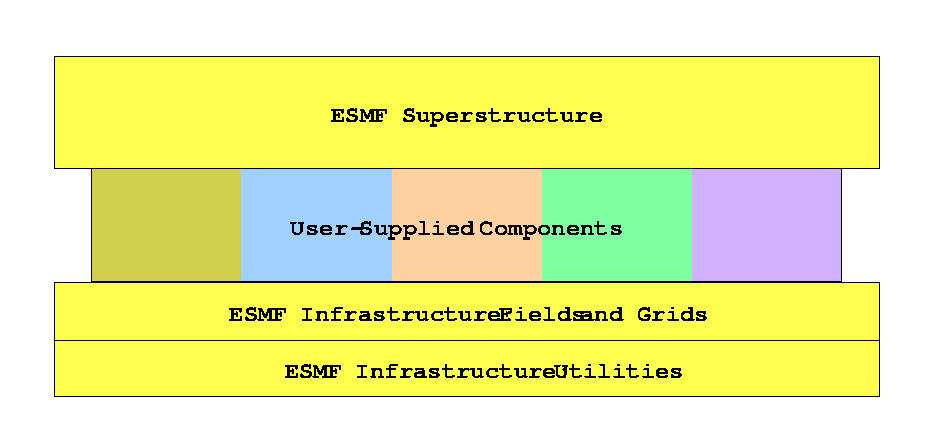
\includegraphics{Sandwich.eps}}
\caption[{ESMF Architecture}] {The simplest view of the ESMF architecture
is that it consists of an infrastructure for developing components and 
a superstructure for assembling applications.}
\label{fig:sandwich}
\end{center}
\end{figure}









%\section{Terminology}
\section{Terminology}

The computers on which large Earth system models run are complex, multi-part
systems that vary considerably in structure, as are Earth system applications 
themselves.  Thus as we begin the task of composing a modular software
infrastructure that incorporates constructs from both computer hardware 
and physical systems, we find that there are a multitude of ways to impose 
categories and layers.  In this section we define a set of terms -- some standard,
some not -- describing alternative ways of deconstructing Earth system applications
and the ESMF.  These terms will help to clarify subsequent discussions.

\subsection{Object-Oriented Design}

The ESMF will be designed using object-oriented (OO) principles.  OO design
is characterized by the use of {\it classes}, and the related strategies of
{\it encapsulation}, {\it inheritance}, and {\it polymorphism}.  Classes 
organize data, attributes, and associated methods into well-defined structures.
Encapsulation means making class data inaccessible so that the underlying representation
can be changed or extended without changing the user interface to the class.
Inheritance allows specialized classes to inherit basic behaviors from generic
classes.  Polymorphism allows a single method to be overloaded for use 
when performing conceptually similar operations.  Together these OO
strategies help to organize and streamline codes, making them more flexible,
maintainable, and extensible.

\subsection{Modes of Parallelism}

We use the term {\bf data parallel} to describe an operation performed
on data that is distributed over multiple memory locations and that typically
represents portions of a single physical quantity.  Roughly the same
calculation occurs on all processors at the same time.  Most individual 
model components are run in a data-parallel fashion.

By {\bf task parallel} we mean operations performed on multiple data sets 
distributed over non-overlapping sets of memory locations.  Typically 
each data 
set represents a different physical system, and the calculations performed
on each set are different as well.

\subsection{Sequencing}

Sequential execution of model components describes the case in which 
one component waits for the other to finish before it begins
to execute.  Components may be in the same or different executables
and may have identical or non-overlapping memory distributions.

Concurrent execution of model components occurs when two components,
whether in the same or different executables, execute simultaneously.

\subsection{Layering Methodologies}

Layering generally refers to a calling hierarchy, in which upper layers 
call lower layers.  While this explains how layers {\it work}, it doesn't 
explain what a layer {\it is}.  In this section we describe some common 
layering approaches.  

We use the term {\bf hardware layering} to refer to a strategy to encapsulate 
programming constructs and tools that reflect the structure of the underlying 
computing environment.  In hardware layering, a bottom layer typically includes 
vendor-specific constructs.  A representative higher layer may automatically 
handle standard operations, such as distributed transposes, that are not  
vendor-specific but still reflect architectural details.  At the application layer 
the user handles objects that represent the application 
domain and not the computing environment.  

Hardware layering is one form of {\bf layering by generality}; general 
tools that can apply to many domains are relegated to bottom layers, 
while domain-specific constructs are in top layers.  This paradigm is
common even in systems running on simpler hardware architectures, where vendor-specific
constructs and other threats to portability and ease of use are not a concern.
Its pervasiveness is simply a reflection of the fact that general tools 
enable a variety of applications to be built upon them.

An alternative view of layers results from combining multiple modes of parallelism 
in a single application.  In Earth system models individual model 
components typically run as data parallel operations.  When a number of 
these are combined in an application such as a coupled climate model, individual 
components or sets of individual components may run as task parallel operations 
on non-overlapping sets of nodes.  Data parallel operations can be viewed
as residing in a lower layer, while the task parallel constructs that 
synchronize and referee data transfers occur at a higher level. We refer to 
this as {\bf task layering}.

Closely related to task layering is the data structure layering used 
in the Weather Research and Forecast (WRF) model.  The top ``driver'' layer 
in this approach specifies data decompositions and controls
the flow of execution.  The lowest ``model'' layer consists of physics routines that
operate on simple arrays.  The middle ``mediation''layer is responsible for 
extracting these simple arrays from the data structures in the driver.
While task layering places domain-specific constructs in lower layers, hardware 
layering place domain-specific constructs in the upper layers.  

Different layering strategies may merely be alternative ways of viewing the same
application; a coupled model can without inconsistency 
be developed both as an application with task layering and with hardware 
layering.  However, some layering strategies are more difficult to reconcile. 
Layering by generality encourages application developers to employ high-level 
data structures in the computational portions of their application codes.  In 
contrast, data structure layering prohibits the application developer from 
incorporating advanced data structures into application codes; instead the
user
programs computations using simple arrays.  The latter approach can simplify coding
when computations are free from communications.  When communications or other
operations that reflect hardware are required within model computations, it 
can be helpful to work with more complex data objects that can encapsulate some
of these details.  POOMA and Overture are examples of frameworks that 
provide such data objects.

The ESMF utility infrastructure and superstructure will utilize hardware layering, and multi-component applications running under ESMF can be viewed as being task-layered.
ESMF does not impose a particular form of layering on component models; both
the WRF model and the POOMA model are supported.












%\section{Decomposition and Data Arrangement}
%\section{Decomposition and Data Arrangement}

The high-performance computers Earth system models run on often include cache hierarchies, 
combinations of shared and distributed memory, and multiple processors.  These architectural features
offer opportunities for performance enhancement through decomposition of work and data.  We 
describe data and memory decomposition in more detail in this section.

\subsection{Machine Model}

We propose a general machine model that consists of the abstractions {\bf heaps, 
links, tasks} and {\bf processors}.  This model can represent cache hierarchies,
clustered architectures, distinctions between vector and scalar architectures,
massively parallel processors, pure shared memory systems, and heterogeneous
distributed systems in a systematic manner.  The machine model is primarily
for use by the framework developer in designing performance portable 
low level communications and computations.  It is not intended to be visible 
to the application developer.

\subsubsection{Data decomposition}
{\bf Data} is decomposed into different portions of computer memory, which we will 
call {\bf heaps}.  Heaps may represent distributed memory, multiple memory
pools within the same physical memory (e.g., a default stack and a user-created
stack), or a cache hierarchy.  Data may be partitioned into multiple heaps 
for a variety of reasons; a common one is that it allows multiple processors to perform calculations simultaneously on different segments of the data.  Heaps may permit their their data to be viewed and/or accessed for computation
by no processing elements (data may need to be transferred to another heap first), by one processing element (the MPP model), or by multiple processing 
elements (the shared memory model).  Data may be replicated on multiple heaps.  Data is transferred between heaps by one or more {\bf links}, each of which
may be assigned -- or may determine through self-testing -- an associated 
bandwidth and latency.  Links between heaps may be one-to-one, one-to-many, or 
many-to-many.   

\subsubsection{Work decomposition}
Computational work is performed by {\bf processors}, which may be assigned
or may determine through self-testing attributes such as processor speed and a scalar or vector type.
A computational workload is split into multiple {\bf tasks} either by simply being divided 
among processors or via threading.  In MPP architectures, such as the Cray T3E, 
each task running on a processor had its own associated memory, and work and data decomposition 
coincided.  On clusters of shared memory machines each processor on a node may have access
to a shared memory pool and tasks may be threaded, with one or more tasks
permitted per processor.  The number of 
tasks allowed per processor is a processor attribute.  

In order to obtain optimal performance, it is useful to retain control over both work and data decomposition, either directly, which can
become complicated, or through a layer of abstraction that simplifies the constructs yet provides
enough access to offer good performance.  The advantage of the proposed architectural view is that it is quite simple and yet comprehensive.  It may be implemented incrementally, leaving more advanced features, such as self-testing to determine characteristics of the computing environment, for future development.

\subsubsection{Expressing Decompositions}

We have seen that decomposition occurs over both heaps and tasks.  Since
a task is always associated with one heap but the reverse may not be true,
we perform decompositions hierarchically, with the heap decomposition
specified first.  Task decomposition may be specified at a high level
and treated much like a data decomposition, with each task assigned its 
own virtual heap.  It is also possible to leave task decomposition 
unspecified and obtain a default configuration, or to specify it at a 
low level, with tasks sharing memory to increase performance or migrating 
across processors for load balancing.  If the ESMF is used to specify 
all task decomposition
that occurs in the same heap, the framework should be able to reconcile 
or flag potential problems that arise from task decomposition at multiple
levels.

\subsection{Local data arrangement}
How data is arranged in local memory can be critical in obtaining optimal 
performance.  Dense, regular field data is represented through the use 
of a basic data type that has tuples in each dimension (first, last, 
length, stride).  Such a detailed specification is useful when data fields are 
interleaved or when switching 
between row and column major languages.  A data representation that can 
capture a wide variety of arrangements has a better chance of being 
able to reference rather than copy data before a communication.  (In
some cases, such as highly segmented data, a copy may be desirable,
but in others it may be efficient to avoid it.)  The application developer
should be able to rely largely on default data arrangement.

It will be useful to create a separate basic data type for sparse 
matrices, using a standard format such as compressed storage row.












%\section{Implementation Language and Language Interoperability Strategy}
\section{Implementation Language and Language Interoperability Strategy}

It is possible to represent the fundamental features of object-oriented 
software -- polymorphism, inheritance and encapsulation -- in a variety of languages, 
including the usual choices for high-performance systems: C, C++ and F90. \footnote{Albeit 
with differing levels of difficulty and effectiveness.}  Perhaps the best evidence for 
this claim is that widely used object-oriented libraries and frameworks have been 
written in each of these languages.  Given the above, we can assume that the architecture 
and design of the ESMF will be largely independent of its implementation language.  We
anticipate being able to interpret the architecture described in this document, expressed
in the Unified Modeling Language, in whatever implementation language is chosen.  The rationale for our decision is presented in the ESMF Implementation Report.







%\section{Classes}
\section{ESMF Classes}

We divide the ESMF classes into two main categories, those associated with the coupling 
superstructure and those that are part of the utility infrastructure.  Superstructure and data 
classes are based on a hierarchical 
calling tree of increasingly abstract data structures that represent the field data associated 
with the physical systems being modeled.  Utility classes are independent 
of the data classes, though they too have a hierarchical structure; higher-level utilities
employ general-purpose tools such as a message log.

In the listing of classes below we provide a description of each class and its function.

\subsection{Object Model}

The hierarchy of data classes in ESMF is shown in the following UML diagrams.  

\scalebox{0.70}{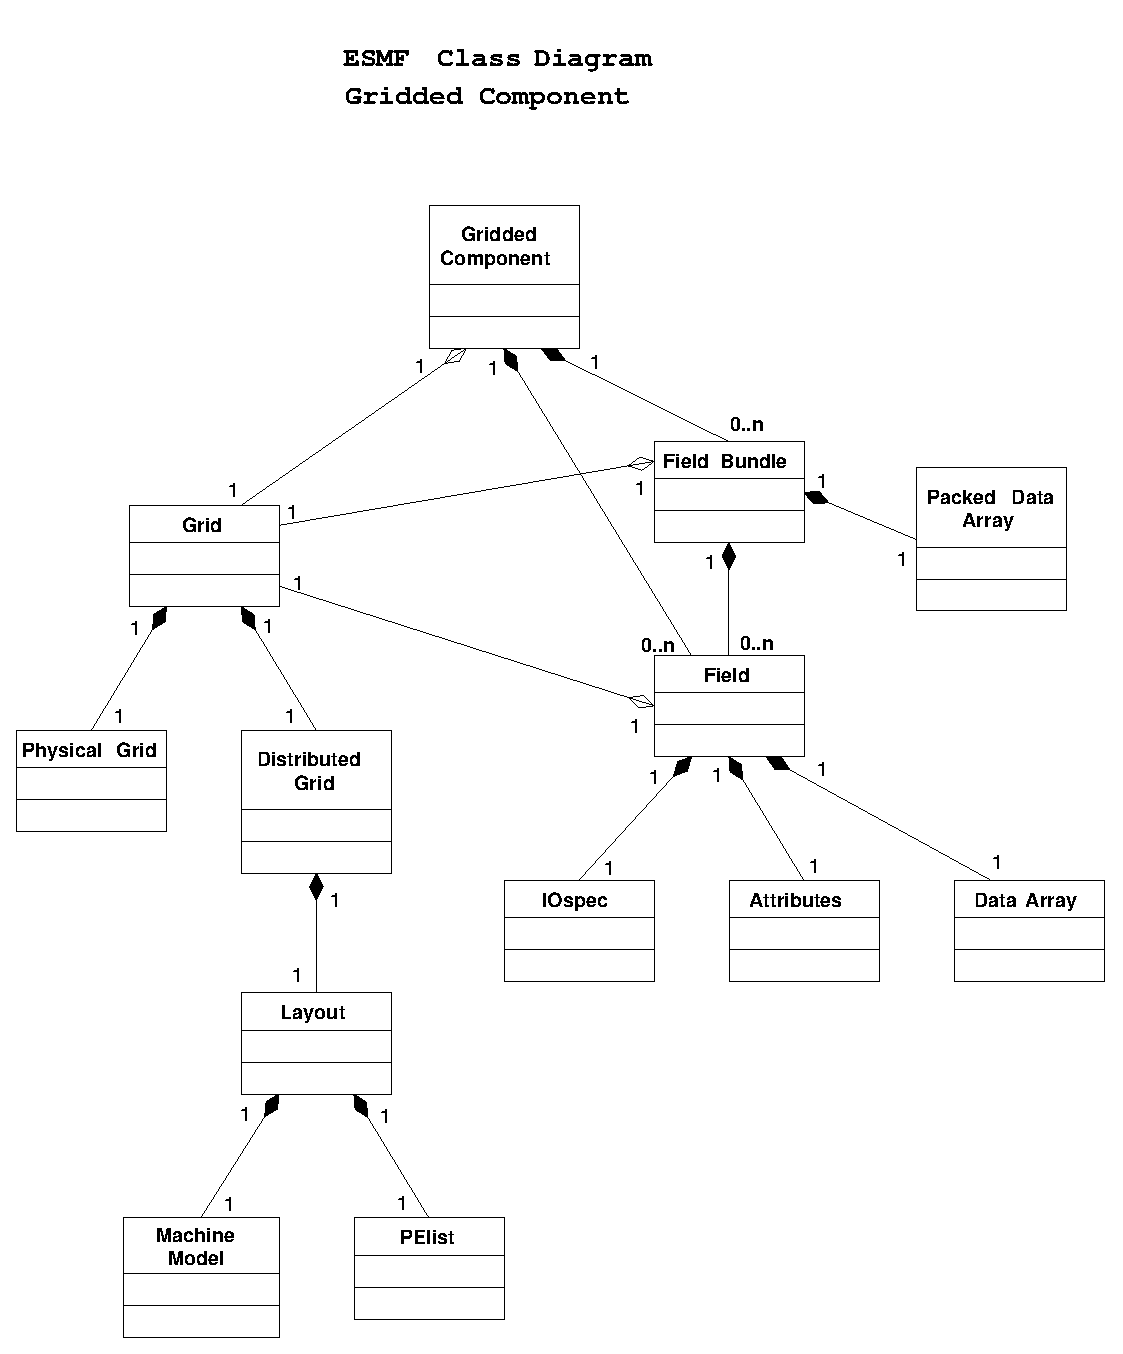
\includegraphics{ESMF_DataStructureHierarchy.eps}}

All objects above are based on the object below.  Attributes
can be handled by generic routines, but it is expected that 
higher level objects will supply their own class specific
methods of the ones listed below.

\scalebox{0.70}{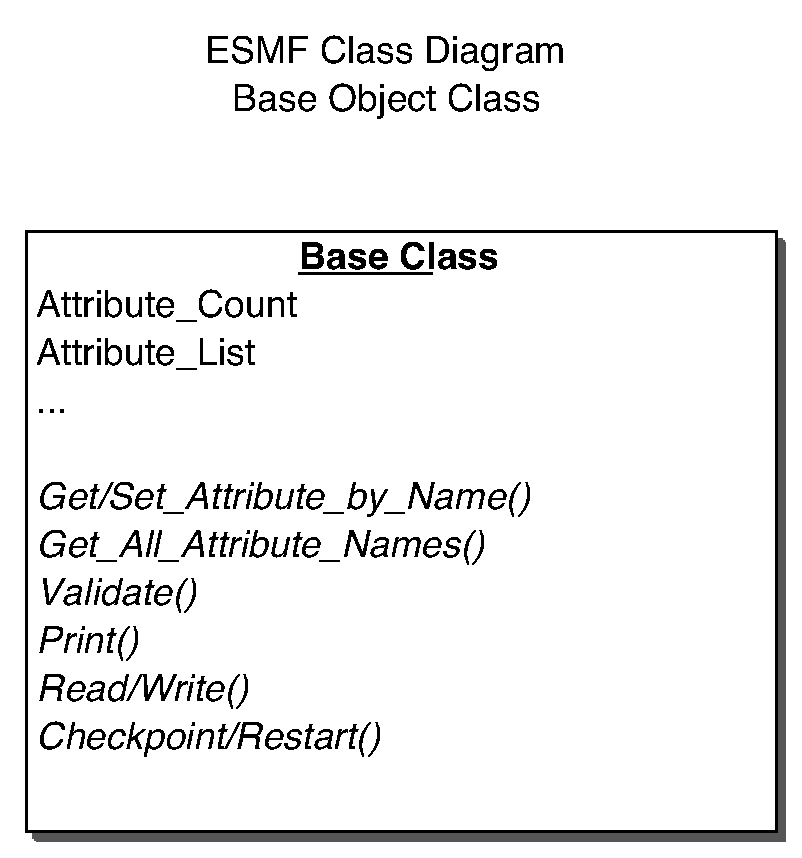
\includegraphics{ESMF_Base.eps}}

Types of components are shown below.

\scalebox{0.70}{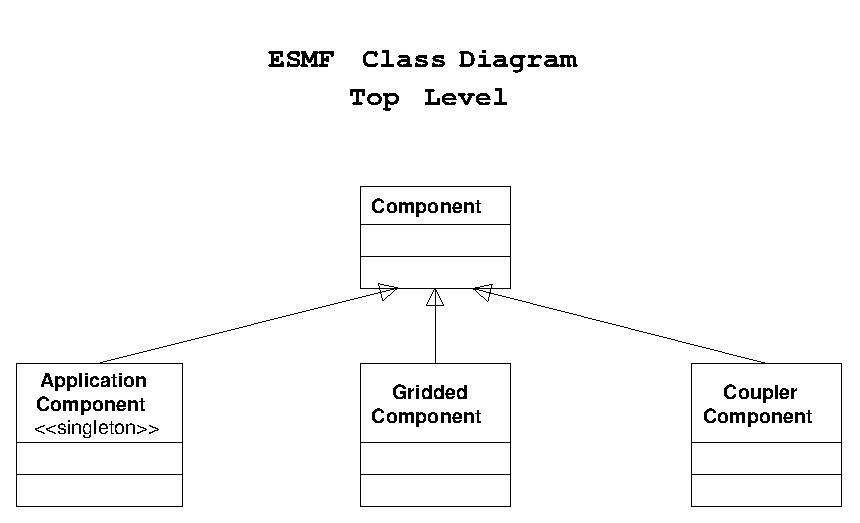
\includegraphics{ESMFTopClassDiagram.eps}}

Coupling diagram.

\scalebox{0.70}{\includegraphics{ESMF_coupler.eps}}

\subsection{Coupling Superstructure}

Below, needs a thorough gutting.

\subsubsection{Component (ESMF\_Comp)} 
\begin{description}
\item [Description] A Component is a functionally related computational entity that represents 
a large system.  
\end{description}

\subsubsection{Application (ESMF\_App)}
\begin{description} 
\item [Description] We define an Application (ESMF\_App) as a special kind of Component 
that is itself composed of a set of sub-Components that interact to form a complete scientific
application.  
\item [Function] The ESMF\_App class is responsible for managing those functions that relate 
to an entire scientific application running under ESMF.  The ESMF\_App initialize method 
must be called at the start of any user application operating under the framework, and
the ESMF\_App finalize method at its end.  At initialization the Application allocates and 
configures any resources needed to run the framework.  The Application also specifies whether 
the system will be brokered using the Registry or not.  The ESMF\_App class can be queried 
for information such as an experiment name, model name, run type (ESMF\_INIT, 
ESMF\_BRANCH, etc.), and for an overall Status.  It can also be queried for
information on any Component that it includes, including its Name, Map, and
Status.
\end{description}

\subsubsection{Coupler Component (ESMF\_Coupler)}
\begin{description}
\item [Description] A Coupler is a specialized type of Component that encompasses all the 
functionality needed to communicate
data between two or more Components. 
\end{description}

\subsubsection{Gridded Component (ESMF\_GComp)} 
\label{sec:gridcomp}
\begin{description}
\item [Description] A Gridded Component is a specialized type of Component that is associated
with a Distributed Grid.  
\end{description}

\subsubsection{Transform (ESMF\_XForm)} 
\begin{description}
\item [Description] A Transform takes one or more physical quantities defined using one set 
of units or representation
and translates them as needed to a different set of units or representation, for example, 
potential temperature
to temperature.  Transform objects are specialized by the application developer.
\item [Function] The Transform class is an abstraction introduced for the
purpose of standardizing high-level coupling interfaces.  It may be overloaded
to take sets of individual Fields or Field Groups.  Methods may include a
separate initialization and run. 
\end{description}

\subsubsection{Layout (ESMF\_Layout)}
\label{sec:layout} 
\begin{description}
\item [Description] A layout is a description of a computational domain that
may describe the decomposition of an Application, a Component, a Field Group, a Field, or 
a Distributed Grid.
If no Layout is specified for an object, it can inherit its layout from an object
higher in the data hierarchy.  
\end{description}

\subsubsection{Distributed Grid (ESMF\_DistGrid)} 

\subsubsection{Field (ESMF\_Field)}
\begin{description} 
\item [Description] A Field represents a single physical field or the components of a 
vector field.  
\end{description}

\subsection{Utility Infrastructure}

\subsubsection{Basic Utilities (ESMF\_BasicUtil)} 
\begin{description}
\item [Description] Utilities that may be utilitized by any other class in the ESMF.  
Collecting these functions into a base-level utility set helps to 
avoid circular referencing.
\item [Function] 
\end{description}

\subsubsection{Basic Communications (ESMF\_BasicComm)}
\begin{description}
\item [Description] This library is a wrapper for MPI and other vendor-supplied 
message passing libraries.
\item [Function] The Basic Communication library provides a generic interface
and efficient communications for the ESMF.  Methods include scatter, gather, send,
receive, synchronize. 
\end{description}

\subsubsection{ (ESMF\_Machine)} 
\begin{description}
\item [Description] The Machine class provides a representation of 
key features of computer hardware and system software.  These
features include memory attributes and configuration, processor type and speed,
interconnect attributes, and system library availability.
\item [Function]
The main purpose of the Machine is to store hardware and system software
information needed by the framework or application programmer in a general
form, but with little abstraction.  This information can be used to perform resource 
allocation, data distribution, and dynamic load balancing.  The Machine can be queried
for platform type(s), number of processors, number of threads, and number of 
nodes.  It may optionally provide information on quantities such as bandwidth and 
latency through active tests.  
\end{description}

\subsubsection{Time Manager (ESMF\_Date, ESMF\_DT)}
\begin{description}
\item [Description] The date and time interval methods in the ESMF provide date
calculations based on a number of different calendars.

\end{description}


















\section{Review Status}

\noindent{\bf Architecture Review} \\

\begin{tabular}{r p{1.3in} p{2in}}
{\bf Review Date:} & <Date> \\ \\
{\bf Reviewers:}   & <Reviewer>          & <Institution> \\
                   & <Reviewer>          & <Institution> \\
                   & <Reviewer>          & <Institution>
\end{tabular}

%\section{Glossary}
%\input{ESMF_glos}

%\section{Bibliography}
%\bibliography{comp} 
%\bibliographystyle{plain}
%\addcontentsline{toc}{section}{Bibliography}

\end{document}







